\documentclass[11pt,a4paper]{article}

\usepackage[utf8]{inputenc}
\usepackage[T1]{fontenc}
\usepackage{lmodern}
\usepackage[margin=2.5cm]{geometry}
\usepackage{amsmath,amssymb,mathtools}
\usepackage{bm}
\usepackage{dsfont}
\usepackage{parskip}
\usepackage{xcolor}
\usepackage{tikz}
\usetikzlibrary{arrows.meta,calc,positioning,decorations.pathmorphing,patterns}
\usepackage{pgfplots}
\pgfplotsset{compat=1.17}
\usepackage[most]{tcolorbox}
\usepackage{enumitem}
\usepackage{hyperref}
\hypersetup{colorlinks=true,linkcolor=blue!50!black,urlcolor=blue!50!black}

% Boxed key results: the box hugs the equation and is centred on the line
\newtcbox{\keybox}{colback=blue!4,colframe=blue!45!black,boxrule=0.6pt,arc=2pt,
  left=8pt,right=8pt,top=4pt,bottom=4pt,on line}
\newcommand{\boxedeq}[1]{%
  \par\vspace{0.4\baselineskip}%
  {\centering\keybox{$\displaystyle #1$}\par}%
  \vspace{0.4\baselineskip}}

% Bra-ket notation
\newcommand{\ket}[1]{\lvert #1\rangle}
\newcommand{\bra}[1]{\langle #1\rvert}
\newcommand{\ketbra}[2]{\lvert #1\rangle\!\langle #2\rvert}
\newcommand{\expval}[1]{\langle #1\rangle}
\newcommand{\mel}[3]{\langle #1\lvert #2\rvert #3\rangle}
\DeclareMathOperator{\Tr}{Tr}

% Notation
\newcommand{\est}{\Theta}                 % estimator
\newcommand{\vmu}{\bm{\mu}}               % measurement record
\newcommand{\Pmu}{P(\vmu\,|\,\theta)}
\newcommand{\FQ}{F_Q}
\newcommand{\ad}{\hat a^\dagger}
\newcommand{\bd}{\hat b^\dagger}
\newcommand{\ah}{\hat a}
\newcommand{\bh}{\hat b}
\newcommand{\term}[1]{\textsc{#1}}

\title{Quantum Sensing and Metrology\\[0.3em]\large Summary}
\author{Tommaso Bonfanti}
\date{June 2026}

\begin{document}
\maketitle
\tableofcontents
\newpage

% =====================================================================
\section{Mach--Zehnder interferometer}

\begin{center}
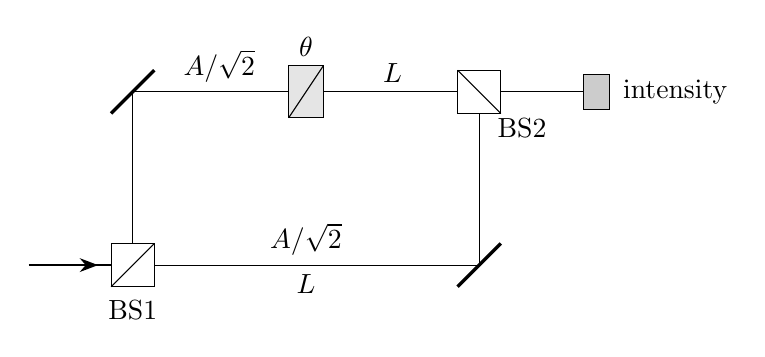
\begin{tikzpicture}[scale=1.1,>=Stealth]
  % beam paths
  \draw[thick] (-1.2,0) -- (0,0);
  \draw[->,thick] (-1.2,0) -- (-0.4,0);
  \draw (0,0) -- (4,0) node[midway,below] {$L$} node[pos=0.5,above] {$A/\sqrt2$};
  \draw (0,0) -- (0,2);
  \draw (0,2) -- (4,2);
  \draw (4,0) -- (4,2);
  \draw (4,2) -- (5.2,2);
  % beam splitters
  \draw[fill=white] (-0.25,-0.25) rectangle (0.25,0.25); \draw (-0.25,-0.25)--(0.25,0.25);
  \node[below] at (0,-0.3) {BS1};
  \draw[fill=white] (3.75,1.75) rectangle (4.25,2.25); \draw (3.75,2.25)--(4.25,1.75);
  \node[below right] at (4.1,1.8) {BS2};
  % mirrors
  \draw[very thick] (-0.25,1.75) -- (0.25,2.25);
  \draw[very thick] (3.75,-0.25) -- (4.25,0.25);
  % phase shifter
  \draw[fill=gray!20] (1.8,1.7) rectangle (2.2,2.3); \draw (1.8,1.7)--(2.2,2.3);
  \node[above] at (2,2.3) {$\theta$};
  \node[above] at (3,2) {$L$};
  \node[above] at (1,2) {$A/\sqrt2$};
  % detector
  \draw[fill=gray!40] (5.2,1.8) rectangle (5.5,2.2);
  \node[right] at (5.55,2) {intensity};
\end{tikzpicture}
\end{center}

We want to measure the phase $\theta$. The output intensity is
\begin{equation*}
  I = \frac12\left|\frac{A}{\sqrt2}e^{ikL} + \frac{A}{\sqrt2}e^{ikL+i\theta}\right|^2
    = \frac{A^2}{2}\left(1+\cos\theta\right).
\end{equation*}

\paragraph{Sensitivity} means: how well can we distinguish $I_{\theta+\delta\theta}$ from $I_\theta$?
\begin{equation*}
  I_{\theta+\delta\theta} \simeq \frac{A^2}{2}(1+\cos\theta) - \frac{A^2}{2}\sin\theta\,\delta\theta .
\end{equation*}
To be able to detect a signal we need $|I_{\theta+\delta\theta}-I_\theta| \geq \Delta I$, with $\Delta I$ the measurement resolution:
\boxedeq{|\delta\theta| \geq \frac{\Delta I}{\frac{A^2}{2}\,|\sin\theta|}}
so that
\[
  \min_\theta |\delta\theta| = \frac{\Delta I}{A^2/2} \qquad\text{at } \theta=\frac{\pi}{2}+n\pi .
\]
To have good sensitivity we want a low $\Delta I$, a large $A$, and $\theta\simeq\pi/2$, i.e.\ we work at the point of maximum slope of $I(\theta)$.

\begin{center}
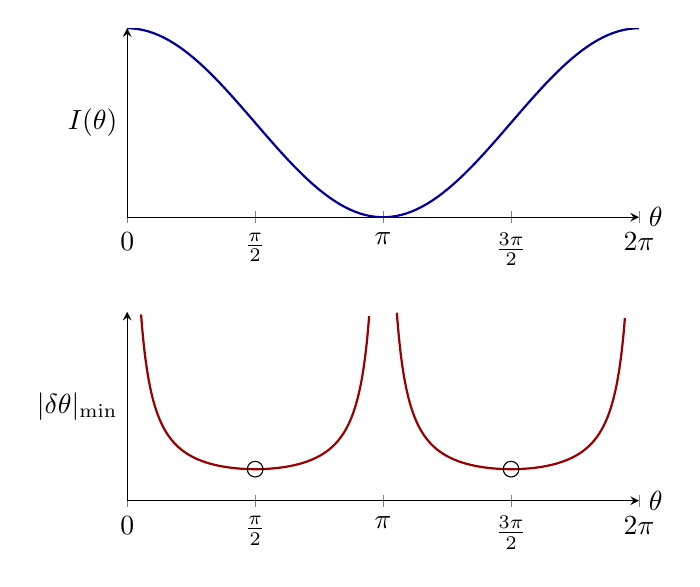
\begin{tikzpicture}
  \pgfplotsset{every axis/.append style={scale only axis,width=6.5cm,height=2.4cm,axis lines=left,
      xmin=0,xmax=6.2832,ytick=\empty,
      xtick={0,1.5708,3.1416,4.7124,6.2832},xticklabels={$0$,$\frac{\pi}{2}$,$\pi$,$\frac{3\pi}{2}$,$2\pi$},
      xlabel={$\theta$},xlabel style={at={(axis description cs:1,0)},anchor=west},
      ylabel style={rotate=-90,anchor=east,at={(axis description cs:0,0.5)}}}}
  \begin{axis}[name=top,ylabel={$I(\theta)$},domain=0:6.2832,samples=100]
    \addplot[thick,blue!60!black] {1+cos(deg(x))};
  \end{axis}
  \begin{axis}[at={(top.south west)},anchor=north west,yshift=-1.2cm,
      ylabel={$|\delta\theta|_{\min}$},ymin=0,ymax=6,samples=200]
    \addplot[thick,red!60!black,domain=0.17:2.97] {1/abs(sin(deg(x)))};
    \addplot[thick,red!60!black,domain=3.31:6.11] {1/abs(sin(deg(x)))};
    \node[draw,circle,inner sep=2pt] at (axis cs:1.5708,1) {};
    \node[draw,circle,inner sep=2pt] at (axis cs:4.7124,1) {};
  \end{axis}
\end{tikzpicture}

{\small Circled: optimal working points, at maximum slope of $I(\theta)$.}
\end{center}

We accomplish this with a bias $\theta_0$:
\[
  I(\theta) = \frac{A^2}{2}\bigl(1+\cos(\theta-\theta_0)\bigr), \qquad \theta_0 \simeq \frac{\pi}{2}+\theta .
\]

\subsection{Standard quantum limit}
Can $\Delta I$ be reduced arbitrarily? A laser is a coherent state $\ket{\alpha}$, with
\[
  \expval{n} = |\alpha|^2 = \bar n, \qquad \Delta n = \sqrt{\bar n}.
\]
The minimum $\Delta I$ we can have, in order to at least distinguish a change in intensity from a random fluctuation, is one standard deviation, $\Delta I\sim\sqrt{\bar n}$. Hence the best possible sensitivity is
\boxedeq{|\delta\theta| \sim \frac{\Delta I}{A^2/2} \sim \frac{\sqrt{\bar n}}{\bar n/2} \sim \frac{1}{\sqrt{\bar n}}
  \qquad \text{(standard quantum limit, SQL)}}

If we try to increase the power, at some point we are limited by the momentum transfer of the photons to the mirrors (radiation pressure):
\[
  F = \frac{2P}{c}, \qquad \Delta F \propto \Delta N \propto \sqrt{\bar n}.
\]
The two contributions, shot noise $\propto 1/\sqrt{\bar n}$ and radiation-pressure noise $\propto\sqrt{\bar n}$, give an optimal photon number:

\begin{center}
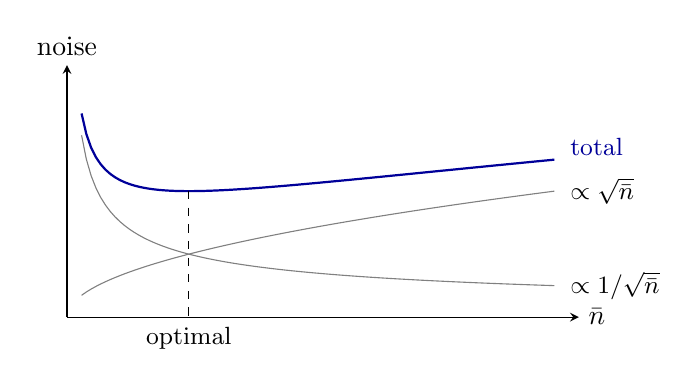
\begin{tikzpicture}
  \begin{axis}[scale only axis,width=6.5cm,height=3.2cm,axis lines=left,clip=false,
      xlabel={$\bar n$},ylabel={noise},xtick=\empty,ytick=\empty,
      domain=0.12:4,samples=100,xmin=0,xmax=4.2,ymin=0,ymax=2,
      xlabel style={at={(axis description cs:1,0)},anchor=west},
      ylabel style={at={(axis description cs:0,1)},anchor=south,rotate=-90}]
    \addplot[thin,gray] {0.5/sqrt(x)};
    \addplot[thin,gray] {0.5*sqrt(x)};
    \addplot[thick,blue!60!black] {0.5/sqrt(x)+0.5*sqrt(x)};
    \node[right,font=\small] at (axis cs:4.05,0.25) {$\propto 1/\sqrt{\bar n}$};
    \node[right,font=\small] at (axis cs:4.05,1.0) {$\propto\sqrt{\bar n}$};
    \node[right,font=\small,blue!60!black] at (axis cs:4.05,1.35) {total};
    \draw[dashed] (axis cs:1,1) -- (axis cs:1,0) node[below,font=\small] {optimal};
  \end{axis}
\end{tikzpicture}
\end{center}

% =====================================================================
\section{Ramsey interferometer}

It is similar to the Mach--Zehnder interferometer. A two-level atom,
\[
  H_0 = E_0\ketbra{0}{0} + E_1\ketbra{1}{1},
\]
passes through three regions:

\begin{center}
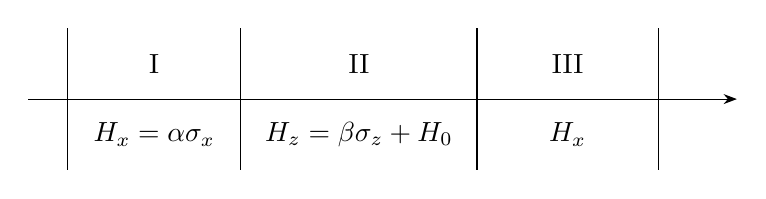
\begin{tikzpicture}[>=Stealth]
  \draw[->] (0,0) -- (9,0);
  \foreach \x in {0.5,2.7,5.7,8} \draw (\x,-0.9) -- (\x,0.9);
  \node at (1.6,0.45) {I};    \node at (1.6,-0.45) {$H_x=\alpha\sigma_x$};
  \node at (4.2,0.45) {II};   \node at (4.2,-0.45) {$H_z=\beta\sigma_z+H_0$};
  \node at (6.85,0.45) {III}; \node at (6.85,-0.45) {$H_x$};
\end{tikzpicture}
\end{center}

On the Bloch sphere, setting $\beta=0$ and $t_3=t_1=\frac{\pi}{4\alpha}$, we have the following procedure:

\begin{center}
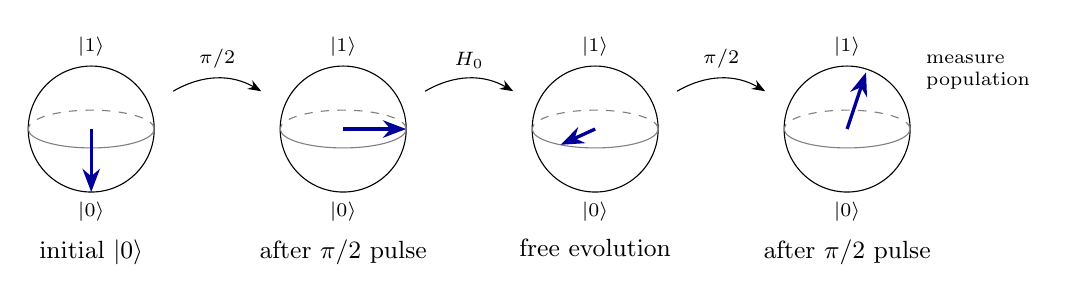
\begin{tikzpicture}[>=Stealth,scale=0.8]
  \newcommand{\bloch}[3]{% center, vector end (relative), label
    \begin{scope}[shift={#1}]
      \draw (0,0) circle (1);
      \draw[gray] (-1,0) arc (180:360:1 and 0.3);
      \draw[gray,dashed] (1,0) arc (0:180:1 and 0.3);
      \node[above,font=\scriptsize] at (0,1) {$\ket1$};
      \node[below,font=\scriptsize] at (0,-1) {$\ket0$};
      \draw[->,very thick,blue!60!black] (0,0) -- #2;
      \node[below,font=\small] at (0,-1.6) {#3};
    \end{scope}}
  \bloch{(0,0)}{(0,-1)}{initial $\ket0$}
  \bloch{(4,0)}{(1,0)}{after $\pi/2$ pulse}
  \bloch{(8,0)}{(-0.55,-0.25)}{free evolution}
  \bloch{(12,0)}{(0.3,0.9)}{after $\pi/2$ pulse}
  \draw[->] (1.3,0.6) to[bend left] node[above,font=\scriptsize] {$\pi/2$} (2.7,0.6);
  \draw[->] (5.3,0.6) to[bend left] node[above,font=\scriptsize] {$H_0$} (6.7,0.6);
  \draw[->] (9.3,0.6) to[bend left] node[above,font=\scriptsize] {$\pi/2$} (10.7,0.6);
  \node[right,font=\scriptsize,align=left] at (13.1,0.9) {measure\\population};
\end{tikzpicture}
\end{center}

Similarly to the MZI, we get
\[
  P(0) = \sin^2\!\left(\frac{(E_1-E_0)\,t_2}{2}\right), \qquad \text{with } \alpha_{\text{opt}} = \frac{\hbar\pi}{4t}.
\]
By measuring the oscillation frequency we can obtain $\Delta E = E_1-E_0$.

% =====================================================================
\section{Classical parameter estimation}

\begin{center}
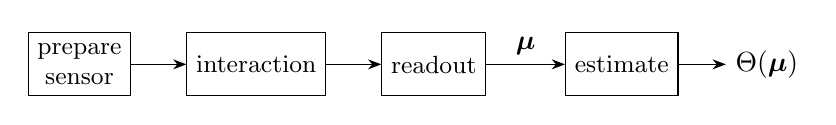
\begin{tikzpicture}[node distance=0.7cm,>=Stealth,
    box/.style={draw,minimum height=0.8cm,align=center,font=\small}]
  \node[box] (p) {prepare\\sensor};
  \node[box,right=of p] (i) {interaction};
  \node[box,right=of i] (r) {readout};
  \node[box,right=1cm of r] (e) {estimate};
  \node[right=0.6cm of e] (t) {$\est(\vmu)$};
  \draw[->] (p) -- (i); \draw[->] (i) -- (r);
  \draw[->] (r) -- node[above] {$\vmu$} (e); \draw[->] (e) -- (t);
\end{tikzpicture}
\end{center}

The experiment is repeated $m$ times to estimate a parameter $\theta$, with i.i.d.\ outcomes. The probability of $\mu_i$ to occur is $P_i(\mu_i|\theta)$, and the \term{likelihood function} is
\[
  \Pmu = \prod_i P_i(\mu_i\,|\,\theta).
\]
To estimate the value of $\theta$ from the measurement results $\vmu$ we construct an \term{estimator} $\est=\est(\vmu)$. Since it is a function of the random variable $\vmu$, it is itself a random variable, so it has a
\begin{itemize}
  \item \textbf{mean value} $\displaystyle \expval{\est} = \bar\est = \sum_{\vmu}\Pmu\,\est(\vmu)$;
  \item \textbf{variance} $\displaystyle (\Delta\est)^2 = \sum_{\vmu}\Pmu\,\bigl(\est(\vmu)-\expval{\est}\bigr)^2$.
\end{itemize}
The discrepancy between estimated and true value is given by the mean squared error
\[
  \text{MSE} = \sum_{\vmu}\Pmu\,\bigl(\est(\vmu)-\theta\bigr)^2
  = \underbrace{\bigl(\expval{\est}-\theta\bigr)^2}_{\text{bias}^2} + (\Delta\est)^2 .
\]
This is the \term{bias--variance tradeoff}: reducing the bias increases the variance.

\subsection{Properties of estimators}
\begin{enumerate}[label=(\roman*)]
  \item \textbf{Unbiased}: if $\expval{\est}=\theta$ $\forall\theta$ (and hence $\partial\bar\est/\partial\theta=1$).
        If this holds only for a large number of measurements, the estimator is called \emph{asymptotically unbiased}.
  \item \textbf{Consistent}: if for $m\to\infty$
        \[ P\bigl(|\est(\vmu)-\theta|\geq\varepsilon\bigr) \to 0 \qquad \forall\varepsilon>0 . \]
        A consistent estimator is asymptotically unbiased.
  \item \textbf{Efficient}: if $\est(\vmu)$ has the lowest possible variance, i.e.\ it saturates the \term{Cramér--Rao bound}:
        \boxedeq{(\Delta\est)^2 \geq \frac{\bigl|\partial\bar\est/\partial\theta\bigr|^2}{F(\theta)}}
\end{enumerate}
where $F$ is the \term{Fisher information}
\[
  F(\theta) = \left\langle\left(\frac{\partial}{\partial\theta}\log\Pmu\right)^2\right\rangle
  = \left\langle -\frac{\partial^2}{\partial\theta^2}\log\Pmu\right\rangle
  = \sum_{\vmu}\frac{1}{\Pmu}\left(\frac{\partial\Pmu}{\partial\theta}\right)^2 .
\]
The FI quantifies how much information the distribution $\Pmu$ carries about $\theta$.
\begin{itemize}
  \item For an unbiased estimator, $(\Delta\est)^2_{\text{CRB}} = 1/F$.
  \item For $m$ independent measurements, $F_{\text{tot}}=\sum_i F_i$.
  \item The CRB can be saturated by an estimator if and only if
        \[
          \frac{\partial}{\partial\theta}\log\Pmu = \lambda\bigl(\est(\vmu)-\expval{\est}\bigr)\quad\forall\vmu,
          \qquad \lambda = \frac{F(\theta)}{\partial\expval{\est}/\partial\theta}.
        \]
\end{itemize}

\subsection{Properties of the Fisher information}
\begin{enumerate}[label=(\alph*)]
  \item \textbf{Convexity}: for $\Pmu=\sum_k\lambda_k P_k(\vmu|\theta)$ with $\lambda_k\geq0$, $\sum_k\lambda_k=1$,
        \[ F(\theta) \leq \sum_k\lambda_k F_k(\theta). \]
  \item \textbf{Additivity}: $F(\theta)=\sum_{i=1}^m F_i(\theta)$ for $m$ measurements.
\end{enumerate}
Since computing $F$ requires full knowledge of $\Pmu$, we can give a lower bound. Consider an observable $M(\mu)$ with $\bar M_\theta=\sum_\mu P(\mu|\theta)M(\mu)$; then
\boxedeq{F(\theta) \geq \frac{1}{(\Delta M)^2}\left(\frac{d\bar M}{d\theta}\right)^2}

\subsection{Maximum likelihood estimator}
\boxedeq{\est_{\text{MLE}}(\vmu) = \operatorname*{arg\,max}_\phi P(\vmu\,|\,\phi)}
Properties of the MLE:
\begin{enumerate}[label=(\roman*)]
  \item \textbf{Consistency}: $\est_{\text{MLE}}(\vmu)\xrightarrow[m\to\infty]{P}\theta$.
  \item \textbf{Efficiency}: the distribution of values $\est_{\text{MLE}}(\vmu)$ tends to a Gaussian with variance $1/F$ by the central limit theorem: $P(\est_{\text{MLE}}|\theta)\to\mathcal G$.
\end{enumerate}
Hence the MLE is asymptotically unbiased, consistent and efficient. It is best when we have a lot of data, i.e.\ when we know $\Pmu$ well.

\subsection{Method of moments}
Consider an observable $M$ with mean $\expval{M}=f(\theta)$ and variance $\Delta M^2$, and the sample average
\[
  M_m = \frac1m\sum_{i=1}^m \mu_i .
\]
By the CLT, $M_m\xrightarrow{m\to\infty}$ Gaussian. The estimator is
\boxedeq{\est_{\text{MOM}} \coloneqq f^{-1}(M_m)}
It is asymptotically unbiased and asymptotically efficient.

\subsection{Bayesian estimation}
This is fundamentally different from the other approaches. We start with a \term{prior} that gives the current knowledge about the true value of a parameter. After a measurement, we update it by computing a \term{posterior} probability through Bayes' theorem:
\[
  \underbrace{P(\phi\,|\,\vmu)}_{\text{posterior}} = \frac{P(\vmu\,|\,\phi)\overbrace{P(\phi)}^{\text{prior}}}{\underbrace{P(\vmu)}_{\text{normalization}}} .
\]
$P(\phi)$ represents the probability that $\phi=\theta$ based on current knowledge. There are different types of estimators:
\begin{itemize}
  \item \textbf{Posterior mean}: $\displaystyle \bar\est_{\text{BE}} = \int_a^b d\phi\,P(\phi|\vmu)\,\phi$;
  \item \textbf{Absolute maximum}: $\displaystyle \est^{\max}_{\text{BE}} = \operatorname*{arg\,max}_{\phi\in[a,b]} P(\phi|\vmu)$ (for a flat prior it is the same as the MLE).
\end{itemize}
From one of these point estimates we can compute the \term{posterior variance}
\[
  (\Delta\phi)^2 \coloneqq \int_a^b d\phi\,P(\phi|\vmu)\bigl(\phi-\est_{\text{BE}}(\vmu)\bigr)^2,
\]
which specifies a confidence interval around $\est_{\text{BE}}$ for a specific measurement sequence $\vmu$. It is different from the estimator variance, which measures how much the output of the estimator fluctuates when repeating the measurements. From $P(\phi|\vmu)$ we can also find confidence intervals $\Omega$:
\[
  P(\phi\in\Omega\,|\,\vmu) = \int_\Omega d\phi\,P(\phi|\vmu).
\]
The Bayesian method is asymptotically consistent and efficient.

We can get a bound that applies to the posterior variance, called the \term{Gosh bound}:
\boxedeq{(\Delta\phi)^2 \geq \frac{1}{G(\vmu)}, \qquad
  G(\vmu) = \int_a^b d\phi\,\frac{1}{P(\phi|\vmu)}\left(\frac{dP(\phi|\vmu)}{d\phi}\right)^2}
It is similar to the CRB, but:
\begin{itemize}
  \item $F(\theta)$ measures how sensitive your measurement is to changes in the parameter; it is a property of the system and does not depend on $\vmu$;
  \item $G(\vmu)$ measures how much information has been extracted by a specific measurement $\vmu$. It is not additive.
\end{itemize}
For $m\to\infty$, the \term{Laplace--Bernstein--von Mises theorem} states that $P(\phi|\vmu)$ becomes a Gaussian centred at the true $\theta$ with variance $1/F(\theta)$, so the Gosh bound $\xrightarrow{m\to\infty}$ CRB.

% =====================================================================
\section{Gravitational wave detection}

In general relativity, mass and energy curve space-time:
\[
  R_{\mu\nu} - \frac12 g_{\mu\nu}R = \frac{8\pi G}{c^4}T_{\mu\nu}.
\]
Distance is expressed as
\[
  ds^2 = \sum_{\mu\nu} g_{\mu\nu}\,dx^\mu dx^\nu ,
\]
which in empty space (Minkowski metric $\eta_{\mu\nu}$) reads
\[
  ds^2 = -c^2dt^2+dx^2+dy^2+dz^2 .
\]
We can expand to linear order, $g_{\mu\nu}=\eta_{\mu\nu}+h_{\mu\nu}$ with $|h_{\mu\nu}|\ll1$, outside the source ($T_{\mu\nu}=0$), and choose a coordinate system such that $h=\operatorname{tr}h_{\mu\nu}=0$:
\[
  -\frac{1}{c^2}\frac{\partial^2}{\partial t^2}h_{\mu\nu} + \nabla^2 h_{\mu\nu} = 0 .
\]
The solutions are plane waves called \term{gravitational waves},
\[
  h_{\mu\nu} = e_{\mu\nu}\,e^{i(\omega t-\mathbf k\cdot\mathbf x)},
\]
with $e_{\mu\nu}$ the polarization tensor. There are two possible polarizations $h_+$, $h_\times$, transverse to the propagation:
\[
  h_{\mu\nu} = \begin{pmatrix} 0&0&0&0\\ 0&h_+&h_\times&0\\ 0&h_\times&-h_+&0\\ 0&0&0&0 \end{pmatrix}.
\]

\subsection{Interferometric detection}
How to measure them? With an interferometer:

\begin{center}
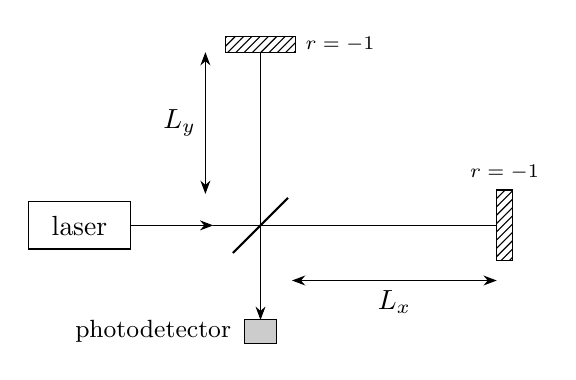
\begin{tikzpicture}[>=Stealth]
  \node[draw,minimum width=1.3cm,minimum height=0.6cm] (las) at (-2.3,0) {laser};
  % beams
  \draw[->] (las.east) -- (-0.6,0);
  \draw (-0.6,0) -- (0,0);
  \draw (0,0) -- (3,0);
  \draw (0,0) -- (0,2.2);
  \draw[->] (0,0) -- (0,-1.2);
  % beam splitter
  \draw[thick] (-0.35,-0.35) -- (0.35,0.35);
  % end mirrors
  \draw[pattern=north east lines] (-0.45,2.2) rectangle (0.45,2.4);
  \node[right,font=\scriptsize] at (0.45,2.3) {$r=-1$};
  \draw[pattern=north east lines] (3,-0.45) rectangle (3.2,0.45);
  \node[above,font=\scriptsize] at (3.1,0.45) {$r=-1$};
  % arm lengths
  \draw[<->] (-0.7,0.4) -- (-0.7,2.2) node[midway,left] {$L_y$};
  \draw[<->] (0.4,-0.7) -- (3,-0.7) node[midway,below] {$L_x$};
  % detector
  \draw[fill=gray!40] (-0.2,-1.5) rectangle (0.2,-1.2);
  \node[left,font=\small] at (-0.25,-1.35) {photodetector};
\end{tikzpicture}
\end{center}

\[
  P \propto E_{\text{out}}^2 = E_0^2\sin^2\bigl(k_L(L_x-L_y)\bigr).
\]
Consider a $(+)$-polarized wave coming from the $z$ direction, $h_+(t)=h_0\cos(\omega_{\text{GW}}t)$:
\begin{gather*}
  ds^2 = -c^2dt^2 + \bigl(1+h_+(t)\bigr)dx^2 + \bigl(1-h_+(t)\bigr)dy^2 + dz^2\\
  \Rightarrow\quad L_x \to L_x\bigl(1+\tfrac12 h_+(t)\bigr),\qquad L_y \to L_y\bigl(1-\tfrac12 h_+(t)\bigr)\\
  \Rightarrow\quad P \propto E_{\text{out}}^2 = E_0^2\sin^2\bigl(k_L L\,h_+(t)+\phi_0\bigr).
\end{gather*}
The intensity oscillates when a GW passes. To increase the sensitivity we increase $L$ with a Fabry--Pérot cavity of finesse $\mathcal F$:
\[
  \tilde L_x = \frac{2}{\pi}\mathcal F L_x, \qquad \mathcal F = \mathcal O(100) \text{ at LIGO}.
\]
We then have the usual bound and the SQL:
\[
  \delta\theta \geq \frac{\Delta I}{\frac{A^2}{2}\,|\sin(\theta-\theta_0)|}, \qquad \delta\theta \sim \frac{1}{\sqrt{\bar n}} .
\]

% =====================================================================
\section{Quantum Mach--Zehnder interferometer}

\begin{center}
\begin{tikzpicture}[>=Stealth]
  \draw[->] (-1.5,2) -- (-0.1,2) node[pos=0,left] {$\hat b_{\text{in}}$};
  \draw[->] (0,3.3) -- (0,2.1) node[pos=0,above] {$\hat a_{\text{in}}$};
  \draw (0,2) -- (3.5,2) -- (3.5,0) -- (0,0) -- (0,2);
  \draw[thick] (-0.3,2.3) -- (0.3,1.7);  % BS1
  \draw[very thick] (3.2,2.3) -- (3.8,1.7); % mirror
  \draw[very thick] (-0.3,0.3) -- (0.3,-0.3); % mirror
  \draw[thick] (3.2,0.3) -- (3.8,-0.3);  % BS2
  \draw[fill=gray!20] (1.55,1.75) -- (1.95,1.75) -- (1.75,2.3) -- cycle;
  \node[above] at (1.75,2.3) {$\theta$};
  \draw[->] (3.5,0) -- (4.6,0) node[right] {$\hat a_{\text{out}}$};
  \draw[->] (3.5,0) -- (3.5,-1.1) node[below] {$\hat b_{\text{out}}$};
\end{tikzpicture}
\end{center}

We use the Heisenberg picture: operators transform, not the quantum states.
\begin{align*}
  \begin{pmatrix}\hat a_{\text{out}}\\ \hat b_{\text{out}}\end{pmatrix}
  &= \underbrace{\frac{1}{\sqrt2}\begin{pmatrix}1&i\\ i&1\end{pmatrix}}_{\text{BS2}}
     \begin{pmatrix}e^{i\theta}&0\\0&1\end{pmatrix}
     \underbrace{\frac{1}{\sqrt2}\begin{pmatrix}1&-i\\ -i&1\end{pmatrix}}_{\text{BS1}}
     \begin{pmatrix}\hat a_{\text{in}}\\ \hat b_{\text{in}}\end{pmatrix}\\
  &= e^{i\theta/2}\begin{pmatrix}\cos\frac\theta2 & \sin\frac\theta2\\ -\sin\frac\theta2 & \cos\frac\theta2\end{pmatrix}
     \begin{pmatrix}\hat a_{\text{in}}\\ \hat b_{\text{in}}\end{pmatrix}.
\end{align*}
We can measure
\[
  \expval{N_{a,\text{out}}} = \expval{\hat a_{\text{in}}^\dagger\hat a_{\text{in}}}\cos^2\frac\theta2 + \expval{\hat b_{\text{in}}^\dagger\hat b_{\text{in}}}\sin^2\frac\theta2,
\]
and similarly for $\expval{N_{b,\text{out}}}$. If $a_{\text{in}}$ has an average of $\bar N$ photons and $b_{\text{in}}$ is vacuum,
\[
  \expval{N_{a,\text{out}}} = \frac{\bar N}{2}(1+\cos\theta), \qquad
  \expval{N_{b,\text{out}}} = \frac{\bar N}{2}(1-\cos\theta),
\]
and with $M=N_{a,\text{out}}-N_{b,\text{out}}$
\[
  \expval{M} = \bar N\cos\theta \quad\Rightarrow\quad
  (\Delta\theta)^2 = \frac{(\Delta M)^2}{\left|\partial\expval{M}/\partial\theta\right|^2}.
\]

% =====================================================================
\section{Ramsey interferometry with spins}

Consider a collection of $N$ spin-$\frac12$ particles with collective spin
\[
  \mathbf J = \sum_{i=1}^N \frac{\bm\sigma^{(i)}}{2}.
\]
A quantum state of the collective spin can be written as
\[
  \ket\psi = \sum_J\sum_m c_{Jm}\ket{J,m}, \qquad J=\tfrac N2,\tfrac N2-1,\dots,\quad m=-J,\dots,J .
\]
The $\ket{J,m}$ are the \term{Dicke states} and they form a basis:
\[
  \mathbf J^2\ket{J,m} = J(J+1)\ket{J,m}, \qquad J_z\ket{J,m} = m\ket{J,m}.
\]
The Ramsey interferometer consists of
\[
  \ket{\psi_{\text{out}}} = e^{i\frac\pi2 J_x}\,e^{-i\theta J_z}\,e^{-i\frac\pi2 J_x}\ket{\psi_{\text{in}}}.
\]
In the Heisenberg picture this is
\[
  \begin{pmatrix}J_x\\J_y\\J_z\end{pmatrix}_{\text{out}}
  = \begin{pmatrix}1&0&0\\0&0&-1\\0&1&0\end{pmatrix}
    \begin{pmatrix}\cos\theta&\sin\theta&0\\-\sin\theta&\cos\theta&0\\0&0&1\end{pmatrix}
    \begin{pmatrix}1&0&0\\0&0&1\\0&-1&0\end{pmatrix}
    \begin{pmatrix}J_x\\J_y\\J_z\end{pmatrix}_{\text{in}},
\]
\[
  \expval{J_z}_{\text{out}} = \cos\theta\expval{J_z}_{\text{in}} - \sin\theta\expval{J_x}_{\text{in}} .
\]
If we use the method of moments with $M=J_{z,\text{out}}$, then $(\Delta\theta)^2=\dfrac{(\Delta M)^2}{(\partial\expval{M}/\partial\theta)^2}$ is easy to find.

\subsection{Schwinger representation}
To unify the Ramsey interferometer and the MZI we use the Schwinger representation:
\[
  J_x = \frac12\left(a^\dagger b + b^\dagger a\right),\qquad
  J_y = \frac1{2i}\left(a^\dagger b - b^\dagger a\right),\qquad
  J_z = \frac12\left(a^\dagger a - b^\dagger b\right),
\]
where from $[a,a^\dagger]=[b,b^\dagger]=1$ we get the SU(2) relations
\[
  [J_k,J_l] = i\varepsilon_{klm}J_m .
\]
The operations in the MZI can now be seen as rotations in spin space:
\[
  \text{BS1: } U=e^{-i\frac\pi2 J_x},\qquad
  \text{BS2: } U=e^{i\frac\pi2 J_x},\qquad
  \text{PS: } U=e^{-i\theta J_z}.
\]
For example, an interferometer with $N$ photons in $a$ and zero in $b$:
\[
  \ket{N}_a\ket{0}_b \;\to\; \ket{J=\tfrac N2,\,m=\tfrac N2}.
\]
Measuring $\expval{J_z}=\frac12\left(\expval{N_a}-\expval{N_b}\right)$ is equivalent to measuring $\expval{M}$.

From $\ket\alpha\ket0$, with $\expval{N_a}=|\alpha|^2$, we get
\[
  (\Delta\theta)^2 = \frac{1}{\expval{N_a}|\sin\theta|^2},
\]
the same as the classical description. With squeezing, in the limit of large $N$, we can beat the SQL $(\Delta\theta)^2\sim1/N$ and get
\[
  (\Delta\theta)^2 \sim \frac{1}{N^{3/2}}
\]
with the same resources, i.e.\ the same total number of photons $N$.

% =====================================================================
\section{Squeezing}

To generate squeezed light, we send it through a nonlinear crystal:
\[
  H = i\hbar g\left(e^{-i\phi}\,\hat a\hat b - e^{i\phi}\,\ad\bd\right).
\]

\begin{center}
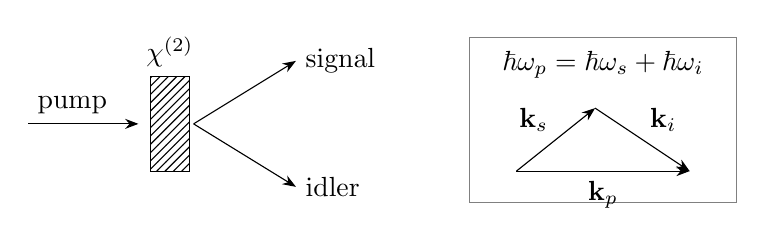
\begin{tikzpicture}[>=Stealth]
  \draw[->] (-1.8,0) -- (-0.4,0) node[pos=0.4,above] {pump};
  \draw[pattern=north east lines] (-0.25,-0.6) rectangle (0.25,0.6);
  \node[above] at (0,0.6) {$\chi^{(2)}$};
  \draw[->] (0.3,0) -- (1.6,0.8) node[right] {signal};
  \draw[->] (0.3,0) -- (1.6,-0.8) node[right] {idler};
  \begin{scope}[shift={(5,0)}]
    \draw[gray] (-1.2,-1) rectangle (2.2,1.1);
    \node at (0.5,0.75) {$\hbar\omega_p=\hbar\omega_s+\hbar\omega_i$};
    \draw[->] (-0.6,-0.6) -- (1.6,-0.6) node[midway,below] {$\mathbf k_p$};
    \draw[->] (-0.6,-0.6) -- (0.4,0.2) node[midway,above left=-1pt] {$\mathbf k_s$};
    \draw[->] (0.4,0.2) -- (1.6,-0.6) node[midway,above right=-1pt] {$\mathbf k_i$};
  \end{scope}
\end{tikzpicture}
\end{center}

Two cases:
\begin{itemize}
  \item \textbf{Degenerate}, $\omega_s=\omega_i$:
  \[
    H = \hbar g'\left(\hat a^{\dagger2}+\hat a^2\right)
    \;\leadsto\; S_1(\xi) = e^{-\frac12\left(\xi^*\hat a^2-\xi\hat a^{\dagger2}\right)}
    \qquad\text{(single-mode squeezing)}
  \]
  where $\xi\sim gt$, $\xi=re^{i\theta}$. The state $\ket\xi=S_1(\xi)\ket0$ has only even Fock states populated.
  \begin{align*}
    \hat a(t) &= \hat a_0\cosh r - i\hat a_0^\dagger e^{i\theta}\sinh r,\\
    \hat a^\dagger(t) &= \hat a_0^\dagger\cosh r + i\hat a_0 e^{-i\theta}\sinh r,
  \end{align*}
  \[
    \Rightarrow\quad (\Delta X)^2 = \frac12 e^{-2r},\qquad (\Delta P)^2 = \frac12 e^{2r}.
  \]
  \item \textbf{Non-degenerate}, $\omega_s\neq\omega_i$:
  \[
    H = \hbar g'\left(\hat a\hat b+\ad\bd\right)
    \;\leadsto\; S_2(\xi) = e^{\left(\xi^*\hat a\hat b-\xi\ad\bd\right)}
    \qquad\text{(two-mode squeezing)}
  \]
  \[
    S_2(\xi)\ket{0} = c_{00}\ket{0,0} + c_{11}\ket{1,1} + \dots
  \]
\end{itemize}

% =====================================================================
\section{SU(1,1) interferometer}

\begin{center}
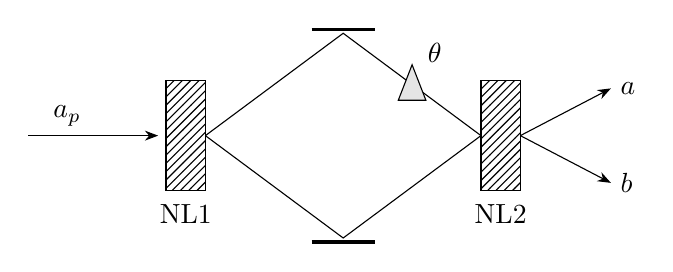
\begin{tikzpicture}[>=Stealth]
  \draw[->] (-2,0) -- (-0.35,0) node[pos=0.3,above] {$a_p$};
  \draw[pattern=north east lines] (-0.25,-0.7) rectangle (0.25,0.7); \node[below] at (0,-0.75) {NL1};
  \draw (0.25,0) -- (2,1.3) -- (3.75,0);
  \draw (0.25,0) -- (2,-1.3) -- (3.75,0);
  \draw[very thick] (1.6,1.35) -- (2.4,1.35);
  \draw[very thick] (1.6,-1.35) -- (2.4,-1.35);
  \draw[fill=gray!20] (2.7,0.45) -- (3.05,0.45) -- (2.875,0.9) -- cycle; \node[above right] at (2.95,0.8) {$\theta$};
  \draw[pattern=north east lines] (3.75,-0.7) rectangle (4.25,0.7); \node[below] at (4,-0.75) {NL2};
  \draw[->] (4.25,0) -- (5.4,0.6) node[right] {$a$};
  \draw[->] (4.25,0) -- (5.4,-0.6) node[right] {$b$};
\end{tikzpicture}
\end{center}

We introduce the operators
\[
  K_x = \frac12\left(a^\dagger b^\dagger + ab\right),\qquad
  K_y = \frac1{2i}\left(a^\dagger b^\dagger - ab\right),\qquad
  K_z = \frac12\left(a^\dagger a + b^\dagger b + 1\right).
\]
These satisfy the SU(1,1) algebra. The conserved quantity is
\[
  K^2 = K_z^2 - K_x^2 - K_y^2 ,
\]
related to the photon-number difference (invariance). Then, instead of the Bloch sphere, states live on the surface of a hyperboloid. The total photon number is not constant.
\[
  \ket{\psi_{\text{out}}} = e^{irK_x}\,e^{-i\theta K_z}\,e^{-irK_x}\ket{\psi_{\text{in}}}.
\]

\begin{center}
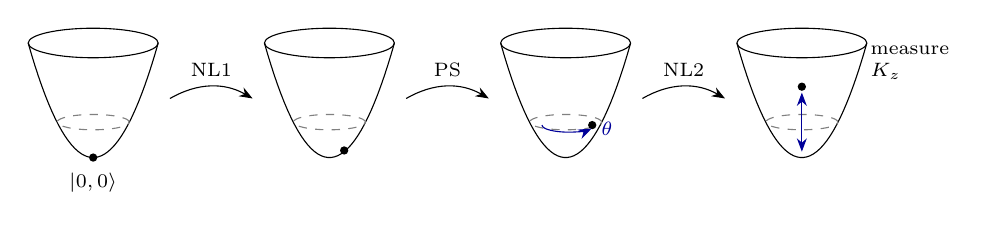
\begin{tikzpicture}[>=Stealth,scale=0.75]
  \newcommand{\hyp}[1]{%
    \begin{scope}[shift={#1}]
      \draw[domain=-1.1:1.1,samples=40] plot (\x,{1.6*\x*\x});
      \draw (0,1.94) ellipse (1.1 and 0.25);
      \draw[gray,dashed] (0,0.6) ellipse (0.61 and 0.13);
    \end{scope}}
  \hyp{(0,0)}  \fill (0,0) circle (2pt); \node[below,font=\scriptsize] at (0,-0.1) {$\ket{0,0}$};
  \hyp{(4,0)}  \fill (4.25,0.12) circle (2pt);
  \hyp{(8,0)}  \fill (8.45,0.55) circle (2pt);
  \draw[->,blue!60!black] (7.6,0.55) arc (180:330:0.45 and 0.12) node[right,font=\scriptsize] {$\theta$};
  \hyp{(12,0)} \fill (12,1.2) circle (2pt); \draw[<->,blue!60!black] (12,0.1) -- (12,1.1);
  \node[right,font=\scriptsize,align=left] at (13,1.6) {measure\\$K_z$};
  \draw[->] (1.3,1) to[bend left] node[above,font=\scriptsize] {NL1} (2.7,1);
  \draw[->] (5.3,1) to[bend left] node[above,font=\scriptsize] {PS} (6.7,1);
  \draw[->] (9.3,1) to[bend left] node[above,font=\scriptsize] {NL2} (10.7,1);
\end{tikzpicture}
\end{center}

% =====================================================================
\section{Quantum parameter estimation}

\begin{center}
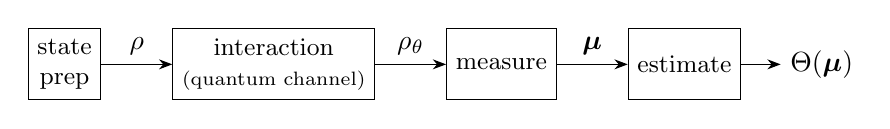
\begin{tikzpicture}[node distance=0.7cm,>=Stealth,
    box/.style={draw,minimum height=0.9cm,align=center,font=\small}]
  \node[box] (p) {state\\prep};
  \node[box,right=0.9cm of p] (i) {interaction\\{\scriptsize(quantum channel)}};
  \node[box,right=0.9cm of i] (m) {measure};
  \node[box,right=0.9cm of m] (e) {estimate};
  \node[right=0.5cm of e] (t) {$\est(\vmu)$};
  \draw[->] (p) -- node[above] {$\rho$} (i);
  \draw[->] (i) -- node[above] {$\rho_\theta$} (m);
  \draw[->] (m) -- node[above] {$\vmu$} (e);
  \draw[->] (e) -- (t);
\end{tikzpicture}
\end{center}

In quantum mechanics, using the Born rule,
\[
  P(\mu\,|\,\theta) = \Tr\left[E_\mu\rho_\theta\right],
\]
where $\{E_\mu\}$ is a POVM:
\[
  \underbrace{\sum_\mu E_\mu = \mathds{1}}_{\text{normalization}},\qquad
  \underbrace{E_\mu\geq0}_{\Rightarrow\,P(\mu|\theta)\geq0} \quad\text{(positive semidefinite)}.
\]
The classical Fisher information is a function of the probability distribution $P(\mu|\theta)$, which now depends on the choice of $\{E_\mu\}$:
\[
  F(\theta) = \sum_\mu\frac{1}{P(\mu|\theta)}\left(\frac{\partial P(\mu|\theta)}{\partial\theta}\right)^2 = F\bigl(\theta,\{E_\mu\}\bigr).
\]
We define the \term{quantum Fisher information}, the absolute maximum of information we can extract:
\boxedeq{\FQ(\theta) = \max_{\{E_\mu\}} F\bigl(\theta,\{E_\mu\}\bigr)
  \qquad\leadsto\qquad
  (\Delta\theta)^2_{\text{QCRB}} \geq \frac{1}{\nu\,\FQ(\theta)}}
with $\nu$ the number of repetitions. In general,
\[
  (\Delta\theta)^2_{\text{exp}} \geq (\Delta\theta)^2_{\text{CRB}} \geq (\Delta\theta)^2_{\text{QCRB}} .
\]

For a \textbf{pure state} undergoing the \textbf{unitary evolution} $U_\theta=e^{-i\theta H}$, where $H$ is the generator of the evolution, we find
\boxedeq{\FQ(\theta) = 4\operatorname{Var}[H]}
In general, for a mixed state the QFI is lower, and for $\rho=\sum_k\lambda_k\ketbra{k}{k}$
\boxedeq{\FQ = 2\sum_{\substack{k,l\\ \lambda_k+\lambda_l\neq0}}\frac{(\lambda_k-\lambda_l)^2}{\lambda_k+\lambda_l}\left|\mel{k}{H}{l}\right|^2}

\subsection{Properties of the QFI}
\begin{enumerate}[label=(\roman*)]
  \item \textbf{Convexity}: if $\rho=\sum_k p_k\rho^{(k)}$ with $p_k\geq0$, $\sum_k p_k=1$,
        \[ \FQ[\rho,H] \leq \sum_k p_k\FQ[\rho^{(k)},H]. \]
  \item \textbf{Additivity}: for $m$ independent subsystems, $\rho=\rho^{(1)}\otimes\dots\otimes\rho^{(m)}$,
        \[ \FQ[\rho,H] = m\,\FQ[\rho^{(1)},H]. \]
\end{enumerate}
For example, for the vacuum state $\operatorname{Var}[X]=\operatorname{Var}[P]=\frac14$. By squeezing one quadrature we get increased sensitivity in the other: for a displacement along $x$,
\[
  \FQ = 4\operatorname{Var}[P],
\]
which can be increased by squeezing.

% =====================================================================
\section{Entanglement and sensitivity}

Consider $N$ identical subsystems, and assume a perturbation that acts locally on each subsystem:
\[
  H = \sum_i h_i \quad\leadsto\quad U = \prod_i e^{-i\theta h_i}.
\]
The max/min eigenvectors and eigenvalues of $h_i$ are $\ket{h_{\max}}$, $h_{\max}$ and $\ket{h_{\min}}$, $h_{\min}$. We consider three cases.

\paragraph{Separable states.}
\[
  \rho_{\text{sep}} = \sum_k p_k\ketbra{\psi^{(k)}_{\text{sep}}}{\psi^{(k)}_{\text{sep}}},\qquad
  \ket{\psi^{(k)}_{\text{sep}}} = \ket{\psi^{(k)}_1}\cdots\ket{\psi^{(k)}_N}.
\]
We find that
\boxedeq{\FQ[\rho_{\text{sep}},H] \leq N\,(h_{\max}-h_{\min})^2}
This is called the \term{standard quantum limit}, and gives a scaling
\[
  (\Delta\theta)^2_{\text{QCRB}} \sim \frac1N .
\]
In this case the optimal state is
\[
  \ket{\psi_{\text{opt}}} = \frac{1}{\sqrt2}\bigl(\ket{h_{\max}}+\ket{h_{\min}}\bigr)
\]
(on each subsystem).

\paragraph{Entangled states.} Consider $\rho=\sum_k p_k\ketbra{\psi^{(k)}}{\psi^{(k)}}$ not separable. We find that, $\forall\rho$,
\boxedeq{\FQ[\rho,H] \leq N^2\,(h_{\max}-h_{\min})^2}
This is called the \term{Heisenberg limit} and gives
\[
  (\Delta\theta)^2_{\text{QCRB}} \sim \frac{1}{N^2}.
\]

\paragraph{Mixture of separable/entangled states.} If $k$ is the size of the largest entangled group, $s=\lfloor N/k\rfloor$ and $r=N-sk$,
\boxedeq{\FQ[\rho,H] \leq \left(sk^2+r^2\right)(h_{\max}-h_{\min})^2}

\begin{center}
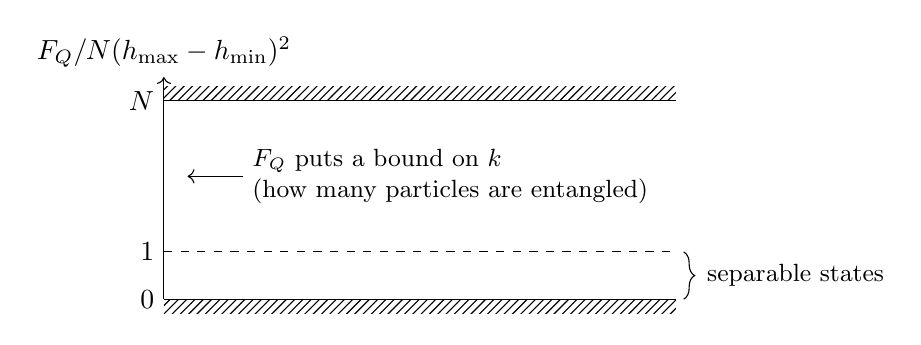
\begin{tikzpicture}[yscale=0.6]
  \fill[pattern=north east lines] (0,4.2) rectangle (6.5,4.5);
  \fill[pattern=north east lines] (0,-0.3) rectangle (6.5,0);
  \draw[->] (0,0) -- (0,4.7) node[above] {$\FQ/N(h_{\max}-h_{\min})^2$};
  \draw (0,0) -- (6.5,0);
  \draw (0,4.2) -- (6.5,4.2);
  \draw[dashed] (0,1) -- (6.5,1);
  \node[left] at (0,0) {$0$};
  \node[left] at (0,1) {$1$};
  \node[left] at (0,4.2) {$N$};
  \draw[decorate,decoration={brace,amplitude=4pt}] (6.6,1) -- (6.6,0) node[midway,right=5pt,font=\small] {separable states};
  \draw[<-] (0.3,2.6) -- (1.0,2.6) node[right,font=\small,align=left] {$\FQ$ puts a bound on $k$\\(how many particles are entangled)};
\end{tikzpicture}
\end{center}

\end{document}
